% !TeX spellcheck = es_ES
\documentclass[12pt]{article} % Default font size is 12pt, it can be changed here
\usepackage[utf8]{inputenc}
\usepackage{geometry} % Required to change the page size to A4
\geometry{a4paper} % Set the page size to be A4 as opposed to the default US Letter
\usepackage{listings}
\usepackage{parskip}
\usepackage{xcolor}
\usepackage{float}
\usepackage{graphicx} % Required for including pictures
\usepackage{hyperref}
\usepackage{float} % Allows putting an [H] in \begin{figure} to specify the exact location of the figure
\usepackage{cite}
\usepackage{fancyhdr}
\usepackage{lscape}
\usepackage{afterpage}
\usepackage[spanish]{babel}
\linespread{1.2} % Line spacing

%\setlength{\parindent}{15pt}
%\setlength\parindent{0pt} % Uncomment to remove all indentation from paragraphs

\graphicspath{{./add/}} % Specifies the directory where pictures are stored

\pagestyle{fancy}
\lhead{Repositorio de árboles genealógicos en BD NoSQL}
\rhead{Daniel Albarral Nuñez}
\cfoot{\thepage}
\renewcommand{\headrulewidth}{0.4pt}
\renewcommand{\footrulewidth}{0.4pt}
\begin{document}

\begin{titlepage}

\newcommand{\HRule}{\rule{\linewidth}{0.5mm}} % Defines a new command for the horizontal lines, change thickness here

\center % Center everything on the page
 
%----------------------------------------------------------------------------------------
%	HEADING SECTIONS
%----------------------------------------------------------------------------------------

\textsc{\LARGE Universidad Politécnica de Cataluña}\\[1.5cm] % Name of your university/college
\textsc{\Large Facultad de Informática de Barcelona}\\[0.5cm] % Major heading such as course name
\textsc{\large Ingeniería de software}\\[0.5cm] % Minor heading such as course 

%----------------------------------------------------------------------------------------
%	TITLE SECTION
%----------------------------------------------------------------------------------------

\HRule \\[0.4cm]
{ \huge \bfseries Repositorio de árboles genealógicos en BD NoSQL}\\[0.4cm] % Title of your document
\HRule \\[1.5cm]
 
%----------------------------------------------------------------------------------------
%	AUTHOR SECTION
%----------------------------------------------------------------------------------------

\begin{minipage}{0.4\textwidth}
\begin{flushleft} \large
\emph{Autor:}\\
Daniel \textsc{Albarral Nuñez} % Your name
\end{flushleft}
\end{minipage}
~
\begin{minipage}{0.4\textwidth}
\begin{flushright} \large
\emph{Director:} \\
Enric \textsc{Mayol} % Supervisor's Name
\end{flushright}
\end{minipage}\\[4cm]

% If you don't want a supervisor, uncomment the two lines below and remove the section above
%\Large \emph{Author:}\\
%John \textsc{Smith}\\[3cm] % Your name

%----------------------------------------------------------------------------------------
%	DATE SECTION
%----------------------------------------------------------------------------------------

%{\large Q1 - 2015-2016}\\[2cm] % Date, change the \today to a set date if you want to be precise

%----------------------------------------------------------------------------------------
%	LOGO SECTION
%----------------------------------------------------------------------------------------


\includegraphics[scale=0.7]{logo_upc.png}\\[1cm] % Include a department/university logo - this will require the graphicx package
 
%----------------------------------------------------------------------------------------

\vfill % Fill the rest of the page with whitespace

\end{titlepage}

%----------------------------------------------------------------------------------------
%   TABLE OF CONTENTS
%----------------------------------------------------------------------------------------

\tableofcontents % Include a table of contents

\newpage % Begins the essay on a new page instead of on the same page as the table of contents 

%----------------------------------------------------------------------------------------
%   Contextualización del proyecto
%----------------------------------------------------------------------------------------
\section{Contextualización del proyecto}

\subsubsection{Los arboles genealógicos}
Un arbole genealógico, también llamado genorama, es la representación gráfica de los antepasados  y descendientes de un individuo.Para su representación  se suelen usar tablas o arboles, siendo esta ultima la forma más común y la que se usara en el proyecto.

\subsubsection{Uso y aplicación de los arboles genealógicos.}
Los arboles genealógicos se usan como herramienta en la genealogía, que se encarga de estudiar y seguir la ascendencia y descendencia de una persona o familia. La genealogía es una ciencia auxiliar de la Historia y es trabajada por un genealogista. Uno de los objetivos del software a desarrollar es dar soporte a los genealogistas. \linebreak Por otro lado hay varias comunidades de aficionados que llevan sus propios arboles genealógicos, el software creado también les podrá dar servicio a esta tipología de usuarios.

\newpage
\subsection{Perspectiva general del software actual.}
Todo software genealógico, como mínimo permite almacenar la siguiente información de un individuo: fecha y lugar de nacimiento, fecha de casamiento, muerte y relaciones familiares, contra más flexible es el programa más información te permite introducir acerca de un individuo. También proporcionan diferentes maneras de representar la información y permiten exportar a GEDCOM la información representada.

\noindent\fbox{\parbox{\textwidth}{\begin{flushleft} GEDCOM \cite{aboutGEDCOM} (\textbf{G}enealogical \textbf{D}ata \textbf{COM}munication):\end{flushleft} Es un formato de archivo de datos, proporciona un formato flexible y uniforme para el intercambio de datos genealógicos computarizados.}}

La mayor parte del software genealógico actual esta basado en soluciones de escritorio, pero en los últimos años han proliferado diferentes soluciones web como myheritage o familysearch, que no solo sirven como plataforma de edición sino que también son grandes plataformas \textit{cloud} en las que se almacenan los arboles genealógicos.

Las soluciones más avanzadas, aparte de la gestión de arboles también ofrecen herramientas más orientadas a la investigación, como podrían ser sistemas de búsqueda de individuos basados en sus relaciones o herramientas estadísticas.

\subsection{Tecnología}
Dada la naturaleza social del tipo de software que se busca desarrollar, nacen ciertas complicaciones tecnológicas que en los últimos tiempos se han sido considerablemente investigadas, debido a la gran repercusión de las redes sociales. Las tecnologías clásicas orientadas a la persistencia de datos como las bases de datos SQL, plantean la dificultad de tener un coste muy alto de consulta cuando se pregunta acerca de datos  con un alto nivel de relación entre ellos. Una de las soluciones más usadas para solucionar este problema son las bases de datos orientadas a grafos, uno de los casos de éxito es el caso de Twitter, que desarrollo su propia solución, FolckDB, una base de datos orientada a grafos, tolerante a fallos, diseñada para tratar con grandes conjuntos de datos, con información no critica.\newline
En el libro \textbf{Neo4j in Action} \cite{neo4jinaction}, Partner and Vukotic realizan el siguiente experimento: \newline
El experimento consiste en comparar una base de datos relacional con neo4j \textit{GraphDB}, en ambas se representa el mismo modelo donde diferentes personas tienen múltiples amigos. Se realizan diferentes consultas donde se pretende averiguar si existe un camino entre dos personas escogidas al azar que los una en una profundidad de como mucho cinco relaciones. Las bases de datos constan de 1000000 personas, cada una con 50 amigos aproximadamente. Los resultados fueron los siguientes:

\begin{figure}[ht!]
\center
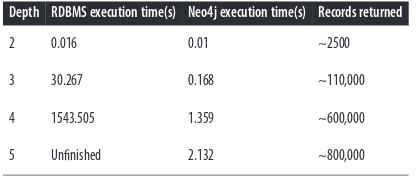
\includegraphics[scale=0.5]{table_find_friends_experiment.png}
\caption{Comparativa entre neo4j y base de datos relacional.}
\label{fig:compa}
\end{figure}

Con este experimento podemos ver como en las consultas donde la profundidad es mayor, o dicho de otra forma, donde la conectividad juega un papel más importante, la base de datos orientada a grafos es mucho más rápida. Esto es debido, en gran parte, a que las relaciones en las bases de datos orientadas a grafos son \textit{ciudadanos de primer orden} a diferencia de las bases de datos relacionales que tratan las relaciones mediante claves foráneas, lo que provoca que tengan que usar una gran cantidad de \textit{joins} para resolver el problema, elevando mucho el coste de resolución.


En el articulo Benchmarking Graph Databases de Alekh Jinda \cite{graphvsrelational} realiza una comparación entre diferentes bases de datos con diferentes naturalezas.

\begin{description}
\item[Neo4j]: Orientada a grafos.
\item[MySQL]: Orientada al tratamiento de filas.
\item[Vertica]: Orientada al tratamiento de columnas.
\item[VoltDB]: Base de datos en memoria principal.
\end{description}

Los conjuntos de datos usados son los siguientes:
\begin{itemize}
\item[-] Conjunto de datos de Facebook, con 4k nodos y 88k aristas.
\item[-] Conjunto de datos de Twitter, con 81k nodos y 1.8M aristas.
\end{itemize}

Las querys aplicadas son \textit{Pagerank} para analizar el comportamiento bajo la necesidad de un \textit{fullscan} y \textit{Dijkstra} para encontrar el camino más corto entre dos nodos. Los resultados los encontramos en la figura \ref{fig:benchmarkingneo4j}

\begin{figure}[ht!]
\center
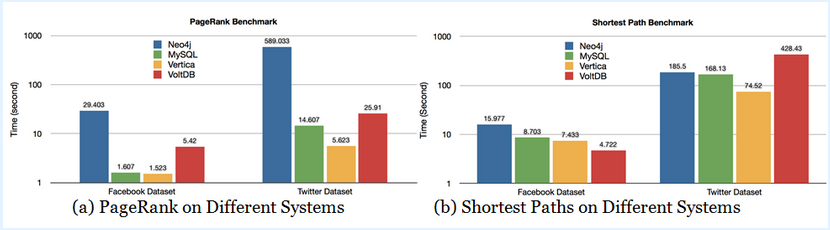
\includegraphics[scale=0.5]{benchmarkingneo4j.png}
\caption{Comparativa entre neo4j y base de datos relacional.}
\label{fig:benchmarkingneo4j}
\end{figure}

Podemos ver que los resultados son contradictorios con el estudio anterior, estaría pendiente de un análisis futuro explicar el por que es estos resultados contradictorios. A pesar de esto neo4j sigue siendo una buena opción, ya que el lenguaje cypher puede facilitar la creación de consultas sobre el modelo a trabajar, dado que un árbol se expresa en forma de grafo de forma natural. También hay que tener en cuenta que este estudio solo examina la rapidez, no el uso de memoria y posiblemente VoldDB al estar orienta a el uso intensivo de memoria principal saldría muy perjudicada.

\subsubsection{Bases de datos orientadas en grafos.}
La gran cantidad de proyectos que han nacido en los últimos años hace prácticamente imposible hacer una comparativa concreta de todas las tecnologías existentes. Pero podemos diferenciar el panorama actual haciendo dos generalizaciones:
\begin{description}
\item[Tecnologías usadas para propósitos transaccionales].\linebreak Orientadas a dar un servicio \textit{online} en tiempo real a una aplicación. Simplifican la diseño del modelo de datos cuando este puede representarse de forma más intuitiva con un grafo. 
\linebreak Estas tecnologías son llamadas \textbf\textit{bases de datos orientadas en grafos}. Son el equivalente a las OLTP en el modelo transaccional.


\noindent\fbox{\parbox{\textwidth}{\begin{flushleft} OLTP (\textbf{O}n\textbf{L}ine \textbf{T}ransaction \textbf{P}rocessing):\end{flushleft} Es un tipo de procesamiento que facilita y administra aplicaciones transaccionales, usualmente para entrada de datos y recuperación y procesamiento de transacciones (gestor transaccional). Los paquetes de software para OLTP se basan en la arquitectura cliente-servidor ya que suelen ser utilizados por empresas con una red informática distribuida..}}

\item[Tecnologías usadas principalmente para el análisis de grafos].\linebreak Llamados \textbf\textit{Motores de procesamiento de grafos}, siguiendo el mismo símil que antes, podríamos pensarlos como herramientas de \textit{data mining} y análisis de procesos(OLAP)
\end{description}

Las bases de datos orientadas en grafos son sistemas de bases de datos que permiten operaciones CRUD (\textit{Create, Read, Update y Delete}) sobre los objetos representados en ellas. Suelen estar orientadas a funcionar con sistemas transaccionales (OLTP), como aviamos mencionado anteriormente. Sus principales propiedades son, las relaciones son \textit{ciudadanos de primer orden}, a diferencia de otros modelos, como el relacional que tienen que usar claves foráneas. En este tipo de base de datos para representar el dominio de nuestro problema simplemente nos b
asta con definir los nodos y las relaciones que lo componen.

En el libro Graph Databases \cite{graphdbbook}, encontramos el siguiente gráfico (Figure \ref{fig:grdb}), que nos da una idea de las principales tecnologías orientadas en grafos y a que enfocan su potencial.

\begin{figure}[ht!]
\center
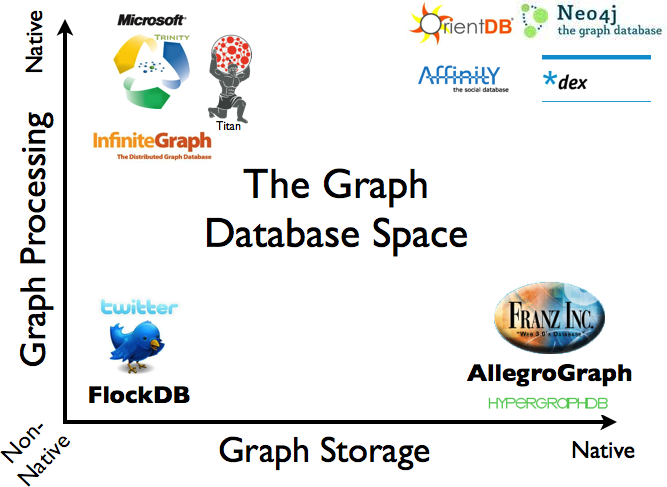
\includegraphics{grdb.png}
\caption{Visión del conjunto de tecnologías}
\label{fig:grdb}
\end{figure}

\newpage
%----------------------------------------------------------------------------------------
%   Metodología y rigor
%----------------------------------------------------------------------------------------
\section{Metodología y rigor}

Las metodologías usadas son las siguientes:

\subsection{SCRUM}
Para el desarrollo del proyecto se ha escogido como metodología de trabajo SCRUM, los \textit{sprints} dado la naturaleza del proyecto se han adaptado esta metodología ágil para ser usada por una sola persona. La metodología de trabajo se ha definido de la siguiente forma:
\begin{description}
	\item[Product backlog]:
	\linebreak Para crear el \textit{product backlog} se han definido un seguido de historias de usuario, de acuerdo con el tutor del proyecto, que asume el rol de \textit{product owner}. Estas historias de usuario se revisaran constantemente en los \textit{sprint backlogs}.
	\item[Sprints]:
	\linebreak Se desarrollaran a lo largo de dos semanas, en este tiempo se desarrollaran las historias de usuario escogidas.
	\item[Sprint backlog]:
	\linebreak Se realizaran al final de cada \textit{sprint}, dado que esta tarea estará limitada por la disponibilidad del tutor y el alumno, se dara flexibilidad pudiendo realizar el \textit{sprint backlog} de varios \textit{sprints} en una reunión. Durante estas reuniones se revisaran las historias de usuario, reorganizando su prioridad, modificando su contenido, añadiendo nuevas o eliminando historias que no se crean necesarias.
\end{description}

\begin{figure}[ht!]
\center
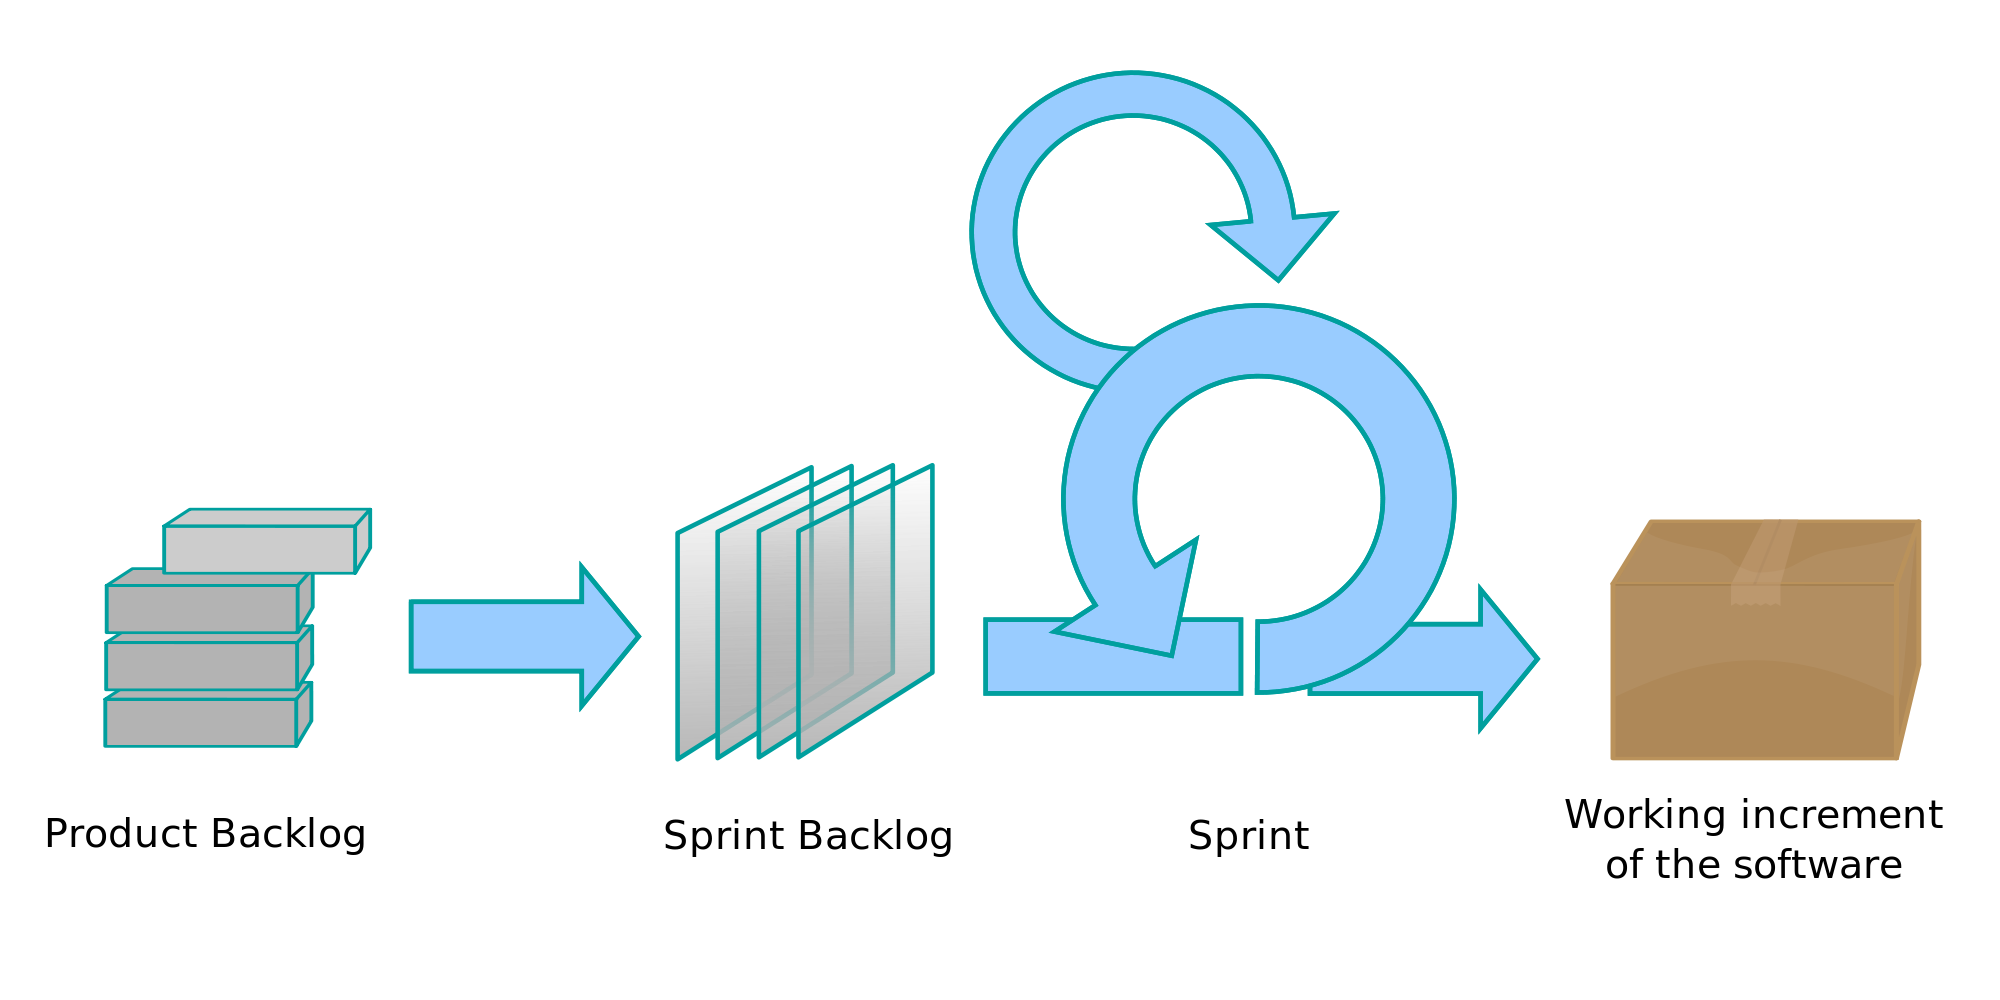
\includegraphics[scale=0.2]{Scrum_process.png}
\caption{Metodología SCRUM}
\label{fig:scrum}
\end{figure}

\subsection{Desviaciones}
Dado al carácter flexible de la metodología, esta no se ha cambiado. Por otro lado durante los \textit{sprints backlogs} se han modificado considerablemente las historias de usuario, lo que ha repercutido en una re-orientación del proyecto, como se explicara en el análisis de alternativas.
\newpage
%----------------------------------------------------------------------------------------
%   Planificación
%----------------------------------------------------------------------------------------

\section{Planificación}
Para el desarrollo del proyecto se usara \textit{Scrum}, por ello la planificación temporal estará estructurada para facilitar la consecución de esta metodología. El final del proyecto se ha establecido el 22 de abril del 2016.

\subsection{Gantt}
El gantt adjuntado a continuación tiene varias peculiaridades:
\begin{description}
\item [Dependencias de las tareas]. 
\linebreak Dado que en el proyecto se desarrolla íntegramente por una sola persona, la secuencialidad del diagrama es absoluta.
\linebreak Durante la fase de desarrollo simplemente se especifican los \textit{Sprints} que se llevaran a cabo hasta conseguir la consecución del proyecto, a medida que las historias de usuario se vayan redactando y priorizando se irán asignando a los \textit{sprints}.
\end{description}

\subsubsection{Tareas y Gráficos gantt}
\begin{landscape}

\begin{figure}[ht!]
\center
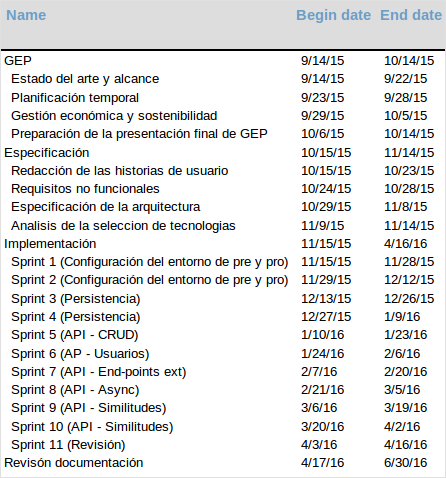
\includegraphics[width=\textwidth,height=\textheight,keepaspectratio]{Task.png}
\label{fig:task}
\end{figure}
\newpage

\begin{figure}[ht!]
\center
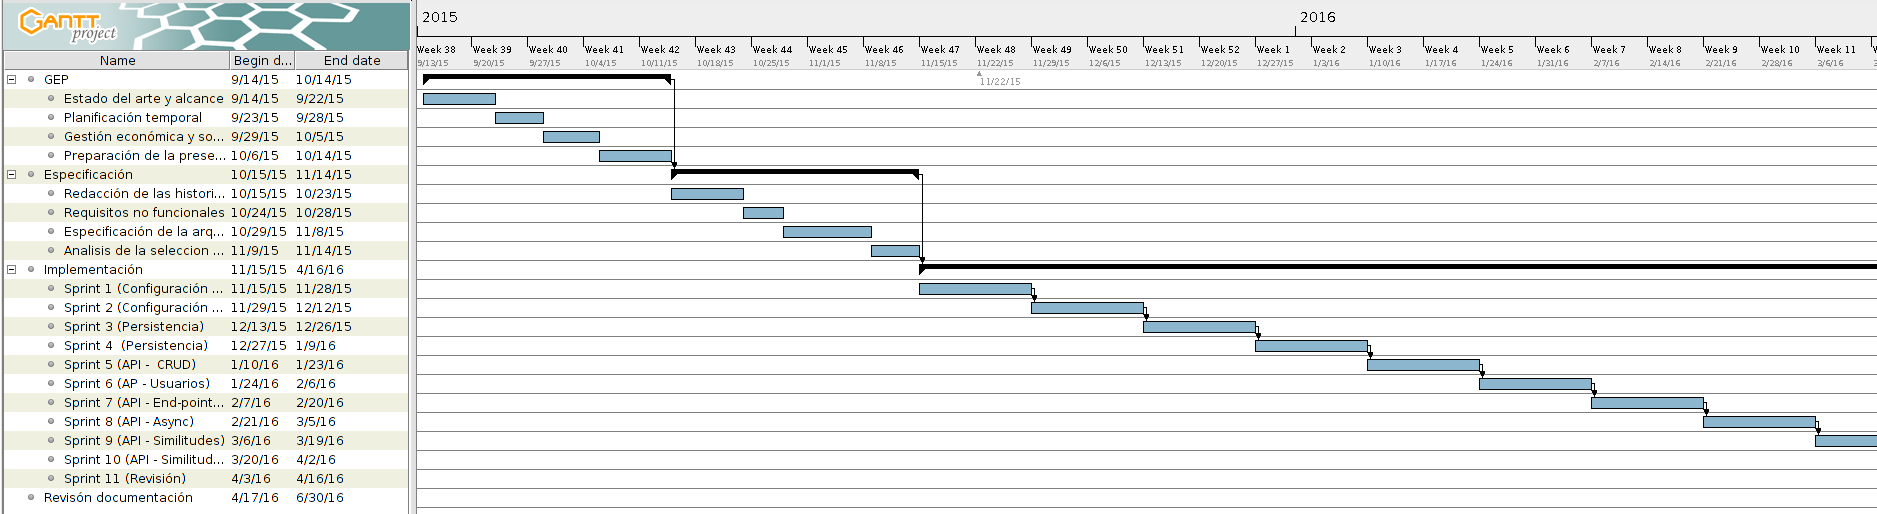
\includegraphics[width=\textwidth,height=\textheight,keepaspectratio]{Gantt_1.PNG}
\label{fig:gantt_1}
\end{figure}

\begin{figure}[ht!]
\center
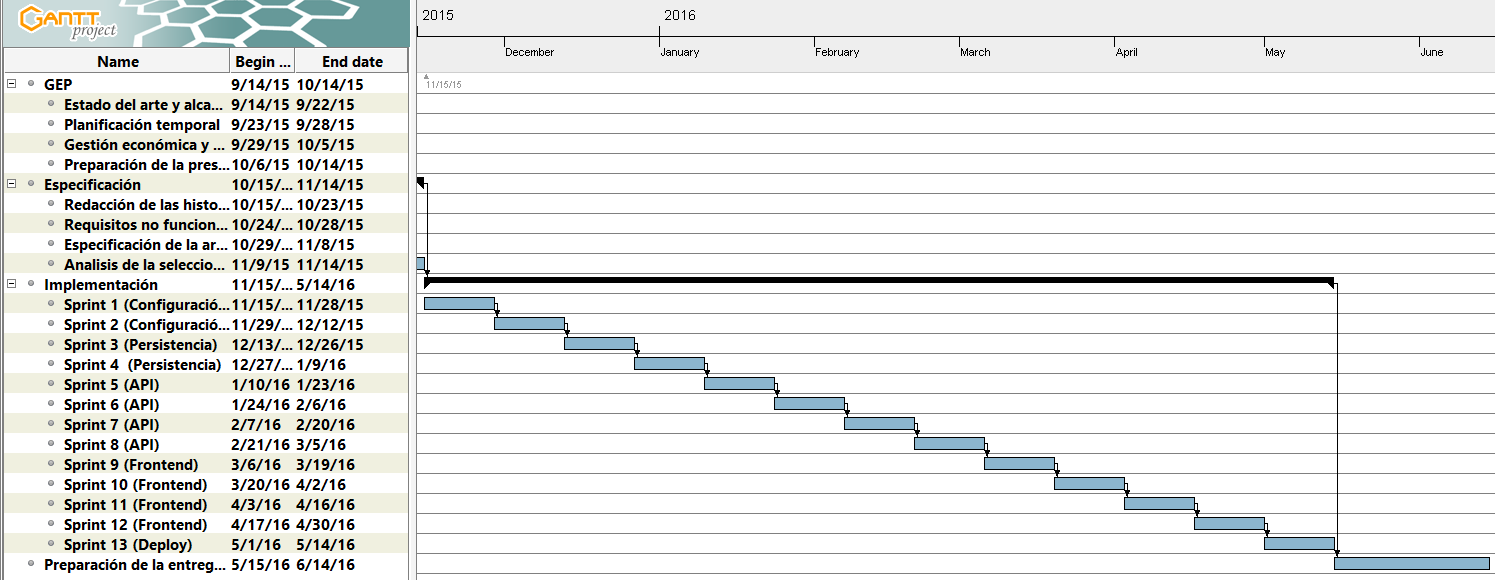
\includegraphics[width=\textwidth,height=\textheight,keepaspectratio]{Gantt_2.PNG}
\label{fig:gantt_2}
\end{figure}

\end{landscape}
\newpage

\subsection{Recursos}
Las necesidades en recursos serán muy escuetas dado que todo el software que se usara es libre y las maquinas en las que se trabaja en pre-producción serán virtuales. La única necesidad de tener unos recursos que se necesiten planificar, ya que requieren ser contratados, son los servidores en los que se hará el \textit{deploy}, se tendrán que contratar durante las semanas que dures los \textit{sprints} en los que se haga el \textit{deploy.} Por otro lado en cuanto a recursos humanos el proyecto se llevara a cabo por un solo desarrollador que se encargar tanto de la programación como la documentación.

\subsection{Alterativas y plan de acción}
Dado que el proyecto se desarrollara usando \textit{Scrum}, al final de cada \textit{sprint}, durante el \textit{sprint backlog} se determinara si se han cumplido las expectativas del \textit{sprint}. Por otro lado en el \textit{sprint planning} se tendrá en cuenta si han habido carencias o \textit{bugs} en los anteriores \textit{sprints} para incorporarlos como historias de usuario al siguiente \textit{sprint}. 

Como se ha comentado en el alcance, se diseñara un software abierto orientado al desarrollo continuado. Por lo que en el \textit{sprint} 13 se dará por concluido el proyecto, y se documentara el estado en el que se encuentre y las historias de usuario pendientes.
\newpage

\subsection{Desviaciones}
Del planteamento inicial del proyecto se ha decidido prescindir del desarrollo del \textit{frontend} y centrar se en la parte del \textit{backend}. Se ha creado \textit{endpoints} asíncronos par las funcionalidades más pesadas y se ha añadido un endpoint para subir archivos GEDCOM.

\subsection{Estado actual de ejecución}
En el punto actual de ejecución del proyecto se da por concluida la implementación de todas las funcionalidades.

%----------------------------------------------------------------------------------------
%   Análisis de alternativas
%----------------------------------------------------------------------------------------
\section{Análisis de alternativas}

%----------------------------------------------------------------------------------------
%¿Se analizan diferentes alternativas para resolver el problema? ¿Se justifica la opción adoptada? Para crear el repositorio de arboles genealogicos, se han identificado diferentes tareas principales y analizado diferentes alternativas:
%----------------------------------------------------------------------------------------

\subsection{Tecnologias}
Se ha establecido como condición necesaria para todas las tecnologías que sean \textit{opensource} o \textit{freeware}. 

\subsubsection{Base de datos}
Se han valorado las siguientes bases de datos:

\begin{description}
\item[HyperGraphDB (\url{http://hypergraphdb.org/})]:
\\Es un base de datos orientada a grafos de propósito general, extensible, potable, distribuida y integrable. Diseñada especialmente para proyectos sobre inteligencia artificial y web semántica. También se pude usar como base de datos orientada a objetos.
\item[InfoGrid (\url{http://infogrid.org})]:
\\Es una base de datos orientada a grafos especialmente enfocada al desarrollo de aplicaciones \textit{backend} REST-ful. Hace especial énfasis en la orientación a objetos. De este proyecto destaca su modularidad. 
\item[Neo4j (\url{http://neo4j.com/})]:
\\Esta base de datos basada en grafos esta diseñada como una base de datos de propósito general, cumple los requisitos de las dos anteriores a pesar que no se pueden crear hyperedges como tal a diferencia de HyperGraphDB, por otro lado se pueden usar técnicas en la representación de los grafos que los simulan. También aporta mejoras en el almacenamiento de los datos respecto a InfoGrid, ya que el almacenamiento esta implementado en grafos de forma nativa.
\end{description}

\textbf{Decisón}:\\
Final mente se ha seleccionado Neo4j. Se ha descartado el uso de HyperGraphDB, dado que pudiéndose acomodar a las necesidades del proyecto no es tan eficiente como InfoGrid y Neo4j cuando usamos la base de datos como una base de datos orientada a objetos puramente.
InfoGrid se ha descartado al no ser tan eficiente como neo4j en el tratamiento de datos en una lógica de grafos, esto se debe a que en InfoGrid los datos no se guardan nativa-mente en estructuras de grafo \cite{neo4jvsinfogrid}.

\subsubsection{Lenguaje de programación}
Los lenguajes escogidos para el análisis han estado seleccionados con criterios subjetivos, seleccionándolos de tal forma que aporten alternativas a la hora tanto de dar agilidad a la implementación como a ser eficientes en el rendimiento. También se ha tendió en cuenta los \textit{frameworks} que se pueden usar en estos lenguajes para la consecución de una API rest.\\Para desarrollar este proyecto se ha optado entre los siguientes lenguajes de programación.

\begin{description}
\item[Scala (\url{www.scala-lang.org/})]:
\\Scala es un lenguaje de propósito general multi-paradigma, da soporte completo para programación funcional y orientada a objetos, también dispone de un sistema de inferencia de tipo estático muy potente. Se compila a Java byte code y se ejecuta sobre la maquina virtual de Java. Es totalmente interoperable con Java por lo que se pueden usar librerías Java y viceversa.

Frameworks:
\begin{description}
\item[Scarlata(\url{www.scalatra.org/})]:
\\Es un \textit{Micro-framework} para scala, consta de librerías para la creación de una API rest completa, como \textit{micro-framework} no fuerza ningún tipo de arquitectura. Se usa para desarrollar bajo la siguiente filosofa:
\begin{description}
\item[Empezar desde lo pequeño, desarrolla hacia arriba]: \\Empieza construyendo un pequeño nucleo y integra módulos simples para solucionar las tareas.
\item[Libertad]: \\Permite al programador usar la estructura y las librerías que crea convenientes para su aplicación.
\item[Solido pero no terco]: \\Usa componentes sólidos para la creación de la API, por ejemplo, los serverlets no son una solución muy moderna a la gestión de la comunicación cliente servidor, pero tienen una gran comunidad detrás y son extremadamente estables. Por otro lado se anima a usar la flexibilidad del framework para usar nuevas técnicas y aproximaciones en diferentes ámbitos del servicio. 
\item[Ama HTTP]: \\HTTP es un protocolo de naturaleza carente de estado, no se ha de pretender usar mecanismos complejos que den la apariencia de estado.
\end{description}

\item[Lift(\url{liftweb.net/})]:
\\Es un \textit{framework} para scala, esta diseñado para seguir la arquitectura 'View First". Clama ser uno de los \textit{frameworks} más seguros y destaca por los siguientes puntos:
\begin{description}
\item[Seguridad]: \\Lift es resistente a casi todas las vulnerabilidades comunes incluyendo la mayoría de la lista ``OWASP \textit{top 10} de".
\item[Amigable para el desarrollador]: \\Lisft esta diseñado para facilitar la creación de aplicaciones de forma rápida y sencilla.
\item[Escalable]: \\Esta diseñado para dar soporte a grandes cantidades de trafico.
\item[Modular]: \\El programa se compone de módulos, esto da mucha agilidad a la hora ampliar las funcionalidades de los proyectos y da una arquitectura muy limpia y fácil de mantener.
\end{description}
\end{description}

\item[Python(\url{python.org/})]:
\\Python es un lenguaje de propósito general, interpretad, y de tipado dinámico. Es un lenguaje multi-paradigma, combina la orientación a objetos con la programación funcional. A diferencia de escala la parte funcional no esta totalmente desarrollada ya que no permitite valores inmutables o técnicas como curring. Python esta diseñado para agilizar el proceso de desarrollo y facilitar la legibilidad y comprensión del código.

Frameworks:
\item[Falsk(\url{flask.pocoo.org/})]:
\\Es un \textit{micro-framework}, esta diseñado permitir el desarrollo de aplicaciones web de forma flexible. Consta de los siguientes herramientas:
\begin{description}
\item[-]Incorpora servidor y debugger
\item[-]Integra soporte para unit test
\item[-]Gestor de peticiones RESTful
\item[-]Usa Jinja2 templating
\item[-]Soporte para ``Cookies'' con seguridad
\item[-]Cumple al 100\% el WSGI 1.0 (Estándar para la comunicación de las aplicaciones con el servidor) 
\item[-]Basado en unicode
\item[-]Extensamente documentado
\end{description}

\item[Django(\url{www.djangoproject.com/})]:
\\Es un \textit{framework}, esta diseñado permitir el desarrollo de aplicaciones rápidamente y con una estructura limpia. Consta de diferentes capas que aportan seguridad la aplicación. Esta basado en la arquitectura modelo vista controlador. Entre sus virtudes destacan la gran facilidad para modular las aplicaciones y facilitar su integración y una comunidad muy extensa, también dispone de una documentación clara, bien estructurada y muy completa. Django destaca en su web estos tres puntos:

\begin{description}
\item[-]Ridicualemtne rapido de desarrollar
\item[-]Altamente seguro
\item[-]Escalabilidad asombrosa
\end{description}
\end{description}

\textbf{Decisión}:
Finalmente se ha escojido Django, ya que es el framework que permite más rapidez en el desarrollo y consta de herramientas que se adhieren altamente a las necesidades del proyecto. A destacar:
\begin{description}
\item[Django Rest Framework]:\\Framework que se integra con Django y proporciona herramientas para facilitar la seralización, enrutamientó teniendo en cuenta el protocolo REST-ful, autorización y autenticación, creación de vistas para las operaciones CRUD, etc.
\item[Django OAuth Toolkit]:\\Conjunto de herramientas para crear autenticación y autorización con permisos, basado en el protocolo oAuth2.
\item[Celerys]:\\Librería de python que permite combinado con una tecnología \textit{``message broker''} permite tarear funcionalidades de la aplicación o crear tareas asíncronas.
\item[neomodel OGM(Object graph maper)]:\\Permite crear modelos en la base de datos neo4j basándose en los modelos de la aplicación.
\end{description}

%----------------------------------------------------------------------------------------
%   Integración de conocimientos
%----------------------------------------------------------------------------------------

\section{Integración de conocimientos}
En el proyecto se integran 3 grandes bloques:

\subsection{Base de datos orientada a grafos}
Se ha diseñado el modelo y de una DB orientada a grafos que represente un árbol genealógico. 
Para la cración del modelo se han usado diferentes técnicas, como los arboles temporales \cite{graphdbbook}. Para las localizaciones se ha creado un sistema que almacena direcciones in-equivocas forma única en forma de árbol, esto se ha conseguido por medio de la API de google maps haciendo uso de los geocomponentes. De esta forma tanto las fechas como las direcciones pueden funciónar como un \textit{``hyperedge''} ya que conseguimos relacionar los diferentes subgrafos por medio de estos nodos.

\subsection{Backend} Creación de un \textit{backend} rest-ful con orientación social, para gestionar la base de datos orientada a grafos. A la hora de construir este \textit{backend} se ha tenido en cuenta patrones arquitectónicos que faciliten la mantenibilidad y ampliabilidad de la aplicación. Este \textit{backend}constara principalmente de:

\subsubsection*{Gestión de usuarios}
Para la gestión de usuarios no se creara ningún \textit{endpoint} en la API por cuestiones de seguridad, se proporcionara una interfaz para poder gestionar los usuarios desde un \textit{frontend }. Los usuarios para darse de alta tendrán que confirmar su correo electrónico.

\subsubsection*{Autorización y autenticación}
Los usuarios, para poder realizar peticiones a los \textit{endpoints} de la API, tendrán que estar autenticados y autorizados, este proceso se hará mediante el protocolo oAuth2, concretamente con \textit{bearer token}.

\subsubsection*{Gestión asincrona}
En los \textit{end-points} más pesados la peticiónes seran asincronias. Esto se conseguira con Rabit MQ como \textit{message broker} y celerys, una librería python que nos permite enviar menssages a la cola de Rabit MQ y gestionar los \textit{workers} que trabajaran sobre ella.

\subsubsection*{Endpoints}
El \textit{backend} consta de todos los \textit{endpoints} necesarios para realizar todas las operaciónes crud sobre el modelo de forma rest-ful. Aparte se incluirán otros \textit{endpoints} para realizar  operaciones adicionales.

\subsection{Busqueda de personas similares}
El programa permitirá encontrar coincidencias entre las personas de la DB. Para ello se aprovechara el potencial de la base de datos orientada a grafos. Para ello se buscaran personas que compartan fechas y lugares en diferentes eventos, nacimiento, muerte, etc. Una vez encontrados estos candidatos se aplicaran heuristicos para determinar en que medida esas dos personas pueden ser la misma.


%----------------------------------------------------------------------------------------
%   Integración de leyes y regulaciones
%----------------------------------------------------------------------------------------
\section{Integración de leyes y regulaciones}
Al desarrollar una aplicación \textit{backend} donde se almacenaran datos de usuarios y personas se tendrá que respetar la \textbf{Ley Orgánica 15/1999 de Protección de Datos de Carácter Personal (Lopd)}. Por ello se tendrá que tener en cuenta:

\subsection{Derecho de información}
El derecho de información esta regulado en la \textbf{Ley Org
ánica 15/1999 de Protección de Datos de Carácter Personal (Lopd)}. Regula las condiciones en que se ha  de recoger, tratar y ceder los datos personales, su fin es proteger la intimidad y demás derechos ciudadanos. Para adecuarse a esta ley, si un usuario introduce datos personales de otra persona se tendrá que se notificar de la posesión de estos datos al afectado y pedir su aprobación para su almacenamiento.

\subsection{Consentimiento del afectado}
EL articulo 6 de la Lopd, regula que para tratar datos personales se ha de tener el consentimiento expreso del damnificado, por ello al registrarse los usuarios tendrán que aceptar una licencia de acuerdo con el usuario final (EULA). Por el momento al ser una plataforma en fase beta donde no se registraran los usuarios no se redactara dicho acuerdo ni se realizara ninguna confirmación a la hora del registro.
\newpage

\bibliography{mybibliography}
\nocite{*}
\bibliographystyle{plain}

\end{document}
